\structure{ХОД РАБОТЫ}

В проекте был написан класс для решения игр с моделью информационного противоборства в социальных сетях.

Пример запуска программы:

\begin{codelisting}[language=Bash]
    go run cmd/lw6/main.go
\end{codelisting}

Сгенерируем стохастическую матрицу доверия для 10 агентов
случайным образом при помощи написанной программы. Вывод программы представлен на рисунке~\ref{fig:fig01}

\begin{figure}
  \centering
  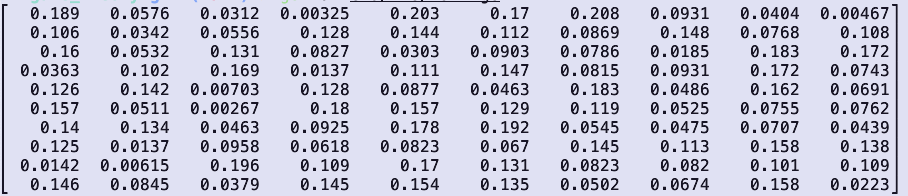
\includegraphics[scale=0.5]{../../artifacts/lw6/1.png}
  \caption{Случайная матрица доверя 10x10}
  \label{fig:fig01}
\end{figure}

Сгенерированный вектор изначальных мнений агентов представлен на рисунке~\ref{fig:fig02}.

\begin{figure}
  \centering
  
\includegraphics[scale=0.6]{../../artifacts/lw6/2.png}
  \caption{Вектор изначальных мнений агентов}
  \label{fig:fig02}
\end{figure}

\section{Нахождение итогового мнения агентов без влияния}

Применим алогоритм согласно формуле (1) с точностью $\mathcal E = 10^{-6}$.

\begin{equation}
\mathbf{x}(t) = A \mathbf{x}(t - 1).
\end{equation}
где $A$ -- случайная матрица доверия, а $x(0)$ -- вектор изначальных мнений агентов.

Спустя 11 итераций алгоритм остановится, так как разница между двумя последними векторами в каждой
координате оказались меньше $10^{-6}$. Вывод итераций представлен на рисунке~\ref{fig:fig03}.

\begin{figure}
  \centering
  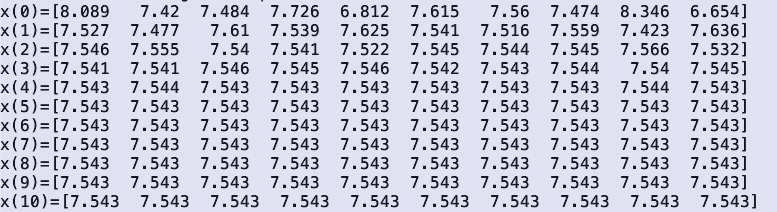
\includegraphics[scale=0.6]{../../artifacts/lw6/3.png}
  \caption{Итерации примененного алоритма}
  \label{fig:fig03}
\end{figure}

После взаимодействия агентов, вектор мнений сходится к значению $7.543$.

Результирующая матрица доверия представлена на рисунке~\ref{fig:fig04}.

\begin{figure}
  \centering
  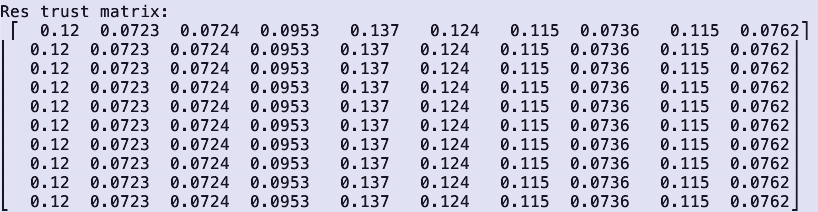
\includegraphics[scale=0.6]{../../artifacts/lw6/4.png}
  \caption{Результирующая матрица доверия}
  \label{fig:fig04}
\end{figure}

\section{Решение игры с информационным влиянием}

Индексы агентов влияния для 2-х игроков представлены на рисунке~\ref{fig:fig05}.

\begin{figure}
  \centering
  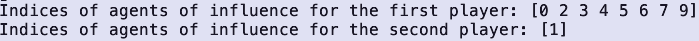
\includegraphics[scale=0.6]{../../artifacts/lw6/5.png}
  \caption{Индексы агентов влияния для 2-х игроков}
  \label{fig:fig05}
\end{figure}

Случайные изначальные мнения для двух игроков представлены на рисунке~\ref{fig:fig06}.

\begin{figure}
  \centering
  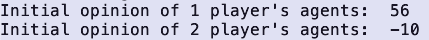
\includegraphics[scale=0.6]{../../artifacts/lw6/6.png}
  \caption{Случайные изначальные мнения для 2-х игроков}
  \label{fig:fig06}
\end{figure}

Аналогично первому пункту, применим алгоритм согласно формуле (1) и остановимся, когда точность не будет
превышать $10^{-6}$. Итерации алгоритма представлены на рисунке~\ref{fig:fig07}.

\begin{figure}
  \centering
  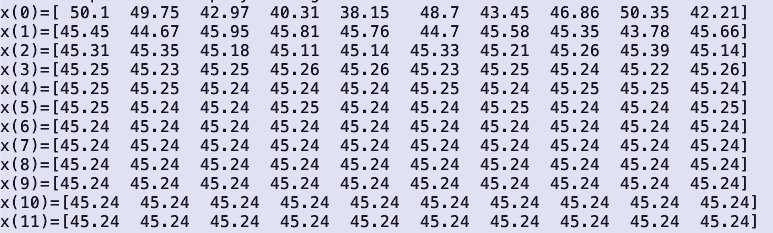
\includegraphics[scale=0.6]{../../artifacts/lw6/7.png}
  \caption{Итерации алгоритма}
  \label{fig:fig07}
\end{figure}

После взаимодействия агентов, вектор мнений сходится к значения, показанный на рисунке~\ref{fig:fig08}

\begin{figure}
  \centering
  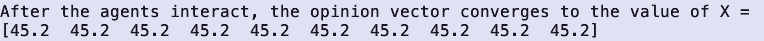
\includegraphics[scale=0.6]{../../artifacts/lw6/8.png}
  \caption{Вектор мнений}
  \label{fig:fig08}
\end{figure}

Найдем расстояния от итогового мнения до изначальных мнений игроков, чтобы определить победителя.

\begin{align*}
  \Delta_1 = \lvert 45.24 - u \rvert = \lvert 45.24 - 56 \rvert = 10.76 \\
  \Delta_2 = \lvert 45.24 - v \rvert = \lvert 45.24 + 10 \rvert = 55.24
\end{align*}

Так как $\Delta_1 < \Delta_2$, то победил первый игрок.
